% ============================================================
%  CSE731 -- Mid-Term Project Report
%  Agentic AI Software Testing Pipeline | IIIT Bangalore
%
%  COMPILE:  pdflatex report.tex   (run TWICE for TOC)
%  Search "TODO" to find placeholders you must fill in.
% ============================================================

\documentclass[12pt, a4paper]{article}

% ── Encoding & Font ─────────────────────────────────────────
\usepackage[T1]{fontenc}
\usepackage[utf8]{inputenc}
\usepackage{lmodern}
\usepackage{microtype}

% ── Page Layout ─────────────────────────────────────────────
\usepackage[
  top=25mm, bottom=28mm,
  left=28mm, right=28mm,
  headheight=14pt
]{geometry}

% ── Colors ──────────────────────────────────────────────────
\usepackage[dvipsnames, table]{xcolor}
\definecolor{PageBg}{HTML}{FDFAF5}
\definecolor{AccentA}{HTML}{2E5F8A}
\definecolor{AccentB}{HTML}{E07B3A}
\definecolor{AccentC}{HTML}{4A9B6F}
\definecolor{CodeBg}{HTML}{F0EDE8}
\definecolor{BoxBg}{HTML}{EBF3FA}
\definecolor{TodoBg}{HTML}{FFF4E6}
\definecolor{SectionColor}{HTML}{1D3F5F}

\usepackage{pagecolor}
\pagecolor{PageBg}

% ── Headers & Footers ───────────────────────────────────────
\usepackage{fancyhdr}
\pagestyle{fancy}
\fancyhf{}
\fancyhead[L]{\small\color{AccentA}\textbf{CSE731} \textemdash{} Agentic AI Testing Pipeline}
\fancyhead[R]{\small\color{AccentA}IIIT Bangalore}
\fancyfoot[C]{\small\color{gray}\thepage}
\renewcommand{\headrulewidth}{0.5pt}

% ── Section Styling ─────────────────────────────────────────
\usepackage{titlesec}
\titleformat{\section}
  {\large\bfseries\color{SectionColor}}
  {\thesection.}{0.5em}{}[{\color{AccentA}\titlerule[0.6pt]}]
\titleformat{\subsection}
  {\normalsize\bfseries\color{AccentA}}
  {\thesubsection}{0.5em}{}
\titlespacing*{\section}{0pt}{14pt}{6pt}
\titlespacing*{\subsection}{0pt}{10pt}{4pt}

% ── Tables ──────────────────────────────────────────────────
\usepackage{booktabs}
\usepackage{tabularx}

% ── Listings (for standalone code blocks only) ───────────────
\usepackage{listings}

\lstdefinestyle{codestyle}{
  language=Python,
  backgroundcolor=\color{CodeBg},
  basicstyle=\ttfamily\footnotesize,
  keywordstyle=\color{AccentA}\bfseries,
  commentstyle=\color{AccentC}\itshape,
  stringstyle=\color{AccentB},
  frame=single,
  framerule=0.5pt,
  rulecolor=\color{gray!40},
  breaklines=true,
  showstringspaces=false,
  tabsize=4,
  numbers=left,
  numberstyle=\tiny\color{gray},
  numbersep=6pt,
  xleftmargin=14pt,
  captionpos=b,
  aboveskip=6pt,
  belowskip=4pt,
}

% ── tcolorbox (with listings library to allow verbatim) ──────
% NOTE: tcbuselibrary{listings} is REQUIRED so that tcblisting
%       can hold verbatim / lstlisting content inside a box.
\usepackage{tcolorbox}
\tcbuselibrary{skins, breakable, listings}

% Shared listing options for prompt boxes
\lstdefinestyle{promptstyle}{
  basicstyle=\ttfamily\scriptsize,
  breaklines=true,
  showstringspaces=false,
  tabsize=2,
  aboveskip=0pt,
  belowskip=0pt,
}

% Prompt box: tcolorbox with built-in listing support
% Usage:  \begin{promptbox}{Title}
%           verbatim text here (no inner \begin{lstlisting} needed)
%         \end{promptbox}
\newtcblisting{promptbox}[1]{
  listing only,
  colback=BoxBg,
  colframe=AccentA,
  colbacktitle=AccentA,
  coltitle=white,
  fonttitle=\bfseries\small,
  title={#1},
  boxrule=0.6pt,
  arc=4pt,
  left=5pt, right=5pt, top=4pt, bottom=4pt,
  breakable,
  listing options={style=promptstyle},
}

% \usepackage[most]{tcolorbox}

\newtcolorbox{codebox}{
    colback=white,
    colframe=orange!70!black,
    colbacktitle=orange!70!black,
    coltitle=white,
    fonttitle=\bfseries,
    title=CLI Command,
    boxrule=0.8pt,
    arc=2pt,
    left=5pt,
    right=5pt,
    top=4pt,
    bottom=4pt
}

% Output box (terminal output style)
\newtcblisting{outputbox}[1]{
  listing only,
  colback=black!4,
  colframe=gray!50,
  colbacktitle=gray!70,
  coltitle=white,
  fonttitle=\bfseries\small,
  title={#1},
  boxrule=0.5pt,
  arc=4pt,
  left=5pt, right=5pt, top=4pt, bottom=4pt,
  breakable,
  listing options={style=promptstyle},
}

% TODO box (no verbatim content -- plain tcolorbox is fine)
\newtcolorbox{todobox}{
  enhanced,
  colback=TodoBg,
  colframe=AccentB,
  colbacktitle=AccentB,
  coltitle=white,
  fonttitle=\bfseries\small,
  title={TODO -- Fill in before submission},
  boxrule=0.7pt,
  arc=4pt,
  left=5pt, right=5pt, top=4pt, bottom=4pt,
  breakable,
}

% Screenshot placeholder box (no verbatim -- plain tcolorbox)
\newtcolorbox{screenshotbox}{
  enhanced,
  colback=white,
  colframe=gray!45,
  boxrule=0.5pt,
  arc=4pt,
  halign=center,
  left=5pt, right=5pt, top=18pt, bottom=18pt,
}

% ── TikZ ────────────────────────────────────────────────────
\usepackage{tikz}
\usetikzlibrary{shapes.geometric, arrows.meta, positioning}

% ── Misc ────────────────────────────────────────────────────
\usepackage{graphicx}
\usepackage{enumitem}
\usepackage{float}
\usepackage{caption}
\usepackage{hyperref}

\captionsetup{font=small, labelfont={bf, color=AccentA}, labelsep=period}
\hypersetup{colorlinks=true, linkcolor=AccentA, urlcolor=AccentB}

\setlength{\parindent}{0pt}
\setlength{\parskip}{6pt}

% ============================================================
\begin{document}
% ============================================================

% ────────────────────────────────────────────────────────────
%  TITLE PAGE
% ────────────────────────────────────────────────────────────
\begin{titlepage}
\begin{center}

\vspace*{12mm}
{\color{AccentA}\rule{\linewidth}{2pt}}
\vspace{5mm}

{\Large\bfseries\color{AccentA}
  International Institute of Information Technology, Bangalore}\\[3mm]
{\normalsize\color{gray} Department of Computer Science and Engineering}

\vspace{8mm}
{\color{AccentB}\rule{0.55\linewidth}{1pt}}
\vspace{10mm}

{\fontsize{21}{27}\selectfont\bfseries\color{SectionColor}
  Agentic AI Software Testing Pipeline}\\[4mm]
{\Large\bfseries\color{AccentB}
  Coverage-Guided Unit Test Generation}

\vspace{8mm}
{\color{AccentA}\rule{0.55\linewidth}{1pt}}
\vspace{10mm}

\begin{tcolorbox}[
  enhanced,
  colback=BoxBg, colframe=AccentA,
  colbacktitle=AccentA, coltitle=white,
  fonttitle=\bfseries, title={Course Information},
  boxrule=0.6pt, arc=4pt, width=0.78\linewidth
]
\begin{tabular}{@{}ll@{}}
  \textbf{Course}  & CSE731: Software Testing              \\[2pt]
  \textbf{Project} & Mid-Term Project, Term I (2026--27)   \\[2pt]
  \textbf{Dataset} & MBPP (Most Basic Python Problems)     \\[2pt]
  \textbf{Model}   & NVIDIA Llama-3.1-Nemotron-70B-Instruct \\
\end{tabular}
\end{tcolorbox}

\vspace{10mm}

{\large\bfseries\color{SectionColor} Team Members}\\[5mm]
\begin{tabular}{cc}
  \toprule
  \rowcolor{AccentA!10}
  \textbf{Name} & \textbf{Roll Number} \\
  \midrule
  Name of Member 1 & IMT2023XXX \\  % TODO: replace
  Name of Member 2 & IMT2023YYY \\  % TODO: replace
  \bottomrule
\end{tabular}

\vfill
{\color{AccentA}\rule{\linewidth}{2pt}}\\[2mm]
{\small\color{gray} Submitted: October 2026}

\end{center}
\end{titlepage}

% ────────────────────────────────────────────────────────────
\tableofcontents
\newpage

% ============================================================
\section{Introduction}
% ============================================================

Unit testing verifies that individual functions behave as expected. This project develops an\textbf{agentic AI pipeline} that automatically generates Python code, produces unit tests targeting a specified coverage criterion, and executes them to obtain measurable testing results. The pipeline is implemented from first principles without RAG, chain-of-thought frameworks, or orchestration libraries such as LangGraph.

\subsection{Objectives}

\begin{itemize}[leftmargin=18pt, itemsep=2pt]
  \item Build a three-agent pipeline:\\
        \textbf{Code Generator} $\to$ \textbf{Test Generator} $\to$
        \textbf{Test Executor}.
  \item Use the \textbf{MBPP} benchmark dataset as the source of problem
        specifications.
  \item Target \textbf{statement and branch coverage} as the testing criterion.
  \item Execute generated tests in an isolated Python environment and obtain a verdict.

\end{itemize}

% ============================================================
\section{Agentic AI Pipeline}
\label{sec:pipeline}
% ============================================================

\subsection{Dataset: MBPP}

The \textbf{Most Basic Python Problems (MBPP)} dataset is a collection of short
Python programming tasks. Each entry contains:

\begin{itemize}[leftmargin=18pt, itemsep=2pt]
  \item A natural-language \emph{prompt} describing the required function.
  \item A \emph{canonical solution} --- the verified, ground-truth implementation.
  \item A small set of \emph{assertion hints} used as specification examples.
\end{itemize}

Tasks are identified by a unique \texttt{task\_id}. The user selects a task via
the CLI using:

\begin{codebox}
\begin{verbatim}
python main.py --task task_id
\end{verbatim}
\end{codebox}

The pipeline then loads the selected task from
\texttt{data/sanitized-mbpp.json}.
\clearpage
\subsection{Pipeline Architecture}

Figure~\ref{fig:pipeline} shows the complete data flow and execution sequence across the three agents.

% ─── PIPELINE DIAGRAM ──────────────────────────────────────
\begin{figure}[H]
\centering
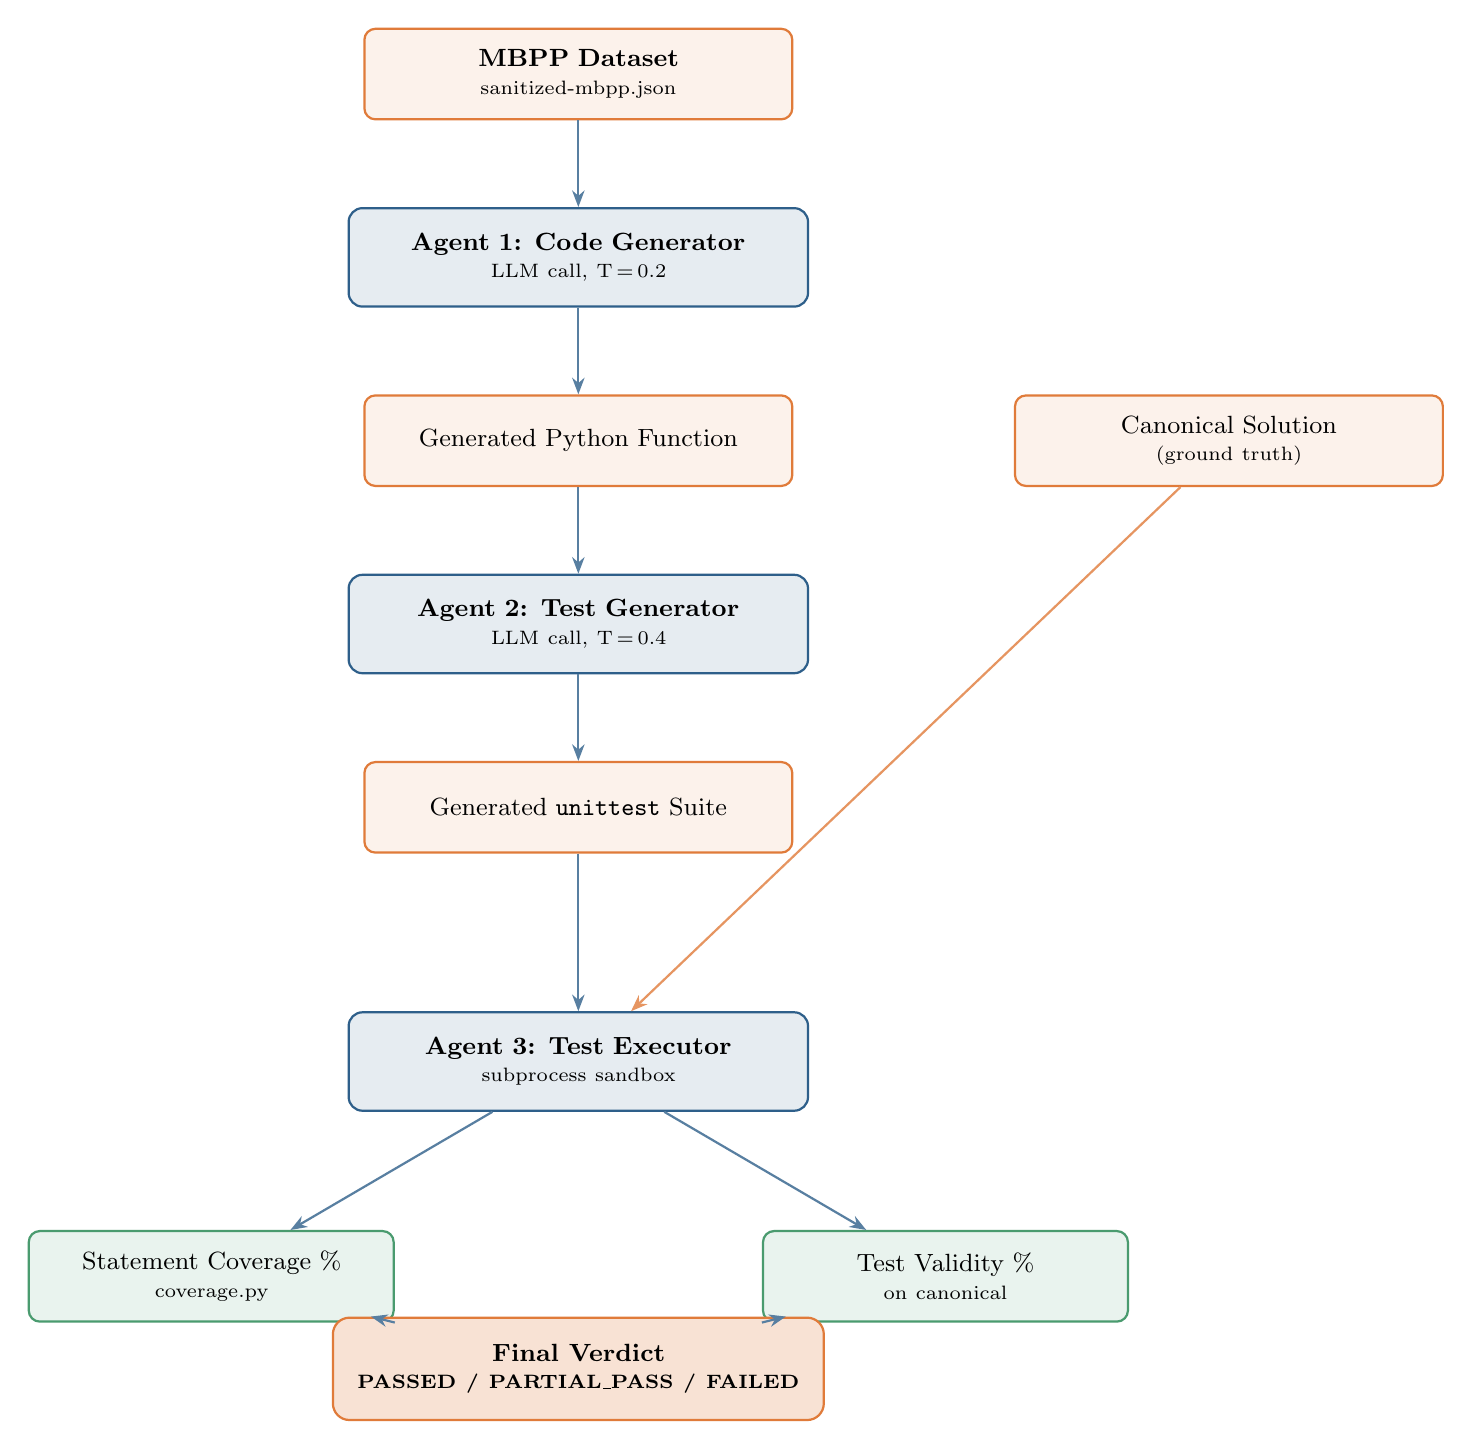
\begin{tikzpicture}[
  font=\small,
  node distance=11mm and 26mm,
  agent/.style={
    rectangle, rounded corners=5pt,
    minimum width=58mm, minimum height=12.5mm,
    text centered, text width=56mm,
    draw=AccentA, fill=AccentA!12, thick
  },
  data/.style={
    rectangle, rounded corners=4pt,
    minimum width=54mm, minimum height=11.5mm,
    text centered, text width=52mm,
    draw=AccentB, fill=AccentB!10, thick
  },
  result/.style={
    rectangle, rounded corners=4pt,
    minimum width=46mm, minimum height=11.5mm,
    text centered, text width=44mm,
    draw=AccentC, fill=AccentC!12, thick
  },
  verdict/.style={
    rectangle, rounded corners=6pt,
    minimum width=62mm, minimum height=13mm,
    text centered, text width=60mm,
    draw=AccentB, fill=AccentB!22, thick, font=\small\bfseries
  },
  arr/.style={-{Stealth[length=6pt]}, thick, color=AccentA!80},
  arr2/.style={-{Stealth[length=6pt]}, thick, color=AccentB!80},
  lbl/.style={font=\scriptsize, color=gray!80},
]

\node[data]   (mbpp) {\textbf{MBPP Dataset}\\[-1pt]
                       {\scriptsize sanitized-mbpp.json}};
\node[agent,  below=of mbpp] (cg)
                      {\textbf{Agent 1: Code Generator}\\[-1pt]
                       {\scriptsize LLM call, T\,=\,0.2}};
\node[data,   below=of cg]   (gc)  {Generated Python Function};
\node[agent,  below=of gc]   (tg)
                      {\textbf{Agent 2: Test Generator}\\[-1pt]
                       {\scriptsize LLM call, T\,=\,0.4}};
\node[data,   below=of tg]   (gt)
                      {Generated \texttt{unittest} Suite};
\node[agent,  below=20mm of gt] (ex)
                      {\textbf{Agent 3: Test Executor}\\[-1pt]
                       {\scriptsize subprocess sandbox}};

\node[data,   right=28mm of gc] (can)
                      {Canonical Solution\\[-1pt]
                       {\scriptsize (ground truth)}};

\node[result, below left=15mm and -6mm of ex]  (cov)
                      {Statement Coverage \%\\[-1pt]
                       {\scriptsize coverage.py}};
\node[result, below right=15mm and -6mm of ex] (val)
                      {Test Validity \%\\[-1pt]
                       {\scriptsize on canonical}};

\node[verdict, below=26mm of ex] (verd)
                      {Final Verdict\\[-1pt]
                       {\scriptsize PASSED / PARTIAL\_PASS / FAILED}};

\draw[arr]  (mbpp) -- (cg);
\draw[arr]  (cg)   -- (gc);
\draw[arr]  (gc)   -- (tg);
\draw[arr]  (tg)   -- (gt);
\draw[arr]  (gt)   -- (ex);
\draw[arr2] (can)  -- (ex);
\draw[arr]  (ex)   -- (cov);
\draw[arr]  (ex)   -- (val);
\draw[arr]  (cov)  -- (verd);
\draw[arr]  (val)  -- (verd);

\end{tikzpicture}
\caption{End-to-end Agentic AI Unit Testing Pipeline.}
\label{fig:pipeline}
\end{figure}

\clearpage

% ─── AGENTS ────────────────────────────────────────────────
\subsection{Agent 1: Code Generator}

The Code Generator Agent receives the problem statement alongside 1-2 example input-output pairs (acceptance criteria from the dataset). This establishes the interface contract (function name and argument types). It also sends a two-part message (system prompt + user prompt) to the LLM and extracts
the returned Python function by stripping Markdown code fences.

\begin{promptbox}{Agent 1 -- System Prompt}
You are an expert Python software engineer.
Write a single, correct Python function that solves the given problem.
Match the expected function name and signature from the examples.
Include any required imports.
Return ONLY the executable Python code inside a ```python ``` block.
\end{promptbox}

\begin{promptbox}{Agent 1 -- User Prompt Template}
Problem Description:
{prompt}

Example assertions:
{test_hints[0]}
{test_hints[1]}

Write the complete Python function implementation:
\end{promptbox}

\vspace{2mm}
\textbf{File:} \texttt{agents/code\_generator.py}

\begin{figure}[H]
\centering
\includegraphics[width=0.95\textwidth]{Agent1.png}
\caption{Agent 1 output -- generated Python function (Task \#2).}
\label{fig:agent1}
\end{figure}

% ─────────────────────────────────────────────────────────────
\subsection{Agent 2: Test Generator}

The Test Generator receives the original prompt and the code from Agent~1.
It generates a \texttt{unittest.TestCase} suite targeting \textbf{maximum statement and
branch coverage}.

\begin{promptbox}{Agent 2 -- System Prompt}
You are an expert Software Test Engineer.
Write unit tests using Python's standard `unittest` framework.
Testing Objective: Maximize statement and branch coverage.
Cover normal paths, edge cases, boundaries, and exceptional values.
Write all test methods inside a class: TestSolution(unittest.TestCase).
Do NOT import from solution files; the function is in the global scope.
Return ONLY executable Python code inside a ```python ``` block.
\end{promptbox}

\begin{promptbox}{Agent 2 -- User Prompt Template}
Problem Description:
{prompt}

Implementation Under Test:
```python
{generated_code}
```

Generate 4 to 8 distinct test methods in TestSolution(unittest.TestCase)
to achieve 100% statement and branch coverage.
\end{promptbox}

\vspace{2mm}
\textbf{File:} \texttt{agents/test\_generator.py}

\begin{figure}[H]
\centering
\includegraphics[width=0.95\textwidth]{Buggy/2Buggy.png}
\caption{Agent 2 output -- generated unittest suite (Task \#2).}
\label{fig:agent2}
\end{figure}

% ─────────────────────────────────────────────────────────────
\subsection{Agent 3: Test Executor and Diagnostic Analyzer}

Agent 3 is divided into two clearly separated phases:

\textbf{Phase 1 --- Offline Execution (no LLM tokens consumed).}
The agent writes the generated code and test suite into a temporary isolated
directory (\texttt{tempfile.TemporaryDirectory}) and executes them in a child
\texttt{subprocess}, ensuring no untrusted code runs in the host process.
Tests are run twice:

\begin{enumerate}
  \item Against the \textbf{canonical (benchmark) solution} to compute
        \emph{Test Validity \%} --- the fraction of generated tests that pass
        on the reference implementation.
  \item Against the \textbf{generated code} with \texttt{coverage.py
        --branch}, producing \emph{Statement Coverage \%} and
        \emph{Generated Pass Rate \%}.
\end{enumerate}

All per-test outcomes (pass, fail, error) and their exact assertion tracebacks
are captured. A 5-second timeout guards against infinite loops.

\textbf{Phase 2 --- Token-Optimised LLM Diagnostic (triggered only on failure).}
After offline execution, a triage gate checks whether any tests failed.
If all tests pass on both solutions, the LLM is \emph{never} called --- zero
tokens are consumed. Only when failures exist does the system send a minimal,
targeted payload to the LLM to diagnose the root cause. The payload is
chosen based on which code failed, as described in
Table~\ref{tab:triage}.

\begin{table}[H]
\centering
\caption{Failure Triage: What is Sent to the LLM and Why}
\label{tab:triage}
\begin{tabular}{>{\raggedright}p{40mm} >{\raggedright}p{58mm} >{\raggedright\arraybackslash}p{42mm}}
\toprule
\rowcolor{AccentA!10}
\textbf{Failure Case} & \textbf{Payload Sent to LLM} & \textbf{Expected Diagnosis} \\
\midrule
Both solutions fail the same test &
  Problem statement + failing test + error &
  Test case is likely wrong or hallucinated \\
\addlinespace
Canonical fails,\newline generated passes &
  Problem statement + canonical code + failing test + error &
  Canonical code missed an edge case (e.g.\ negative inputs) \\
\addlinespace
Generated fails,\newline canonical passes &
  Problem statement + generated code + failing test + error &
  Bug or missing logic in the generated code \\
\addlinespace
All tests pass &
  \emph{Nothing (0 tokens)} &
  No diagnosis needed \\
\bottomrule
\end{tabular}
\end{table}

Figure~\ref{fig:executor} shows the complete flow of Agent 3.

% ─── EXECUTOR FLOWCHART ──────────────────────────────────────
\begin{figure}[H]
\centering
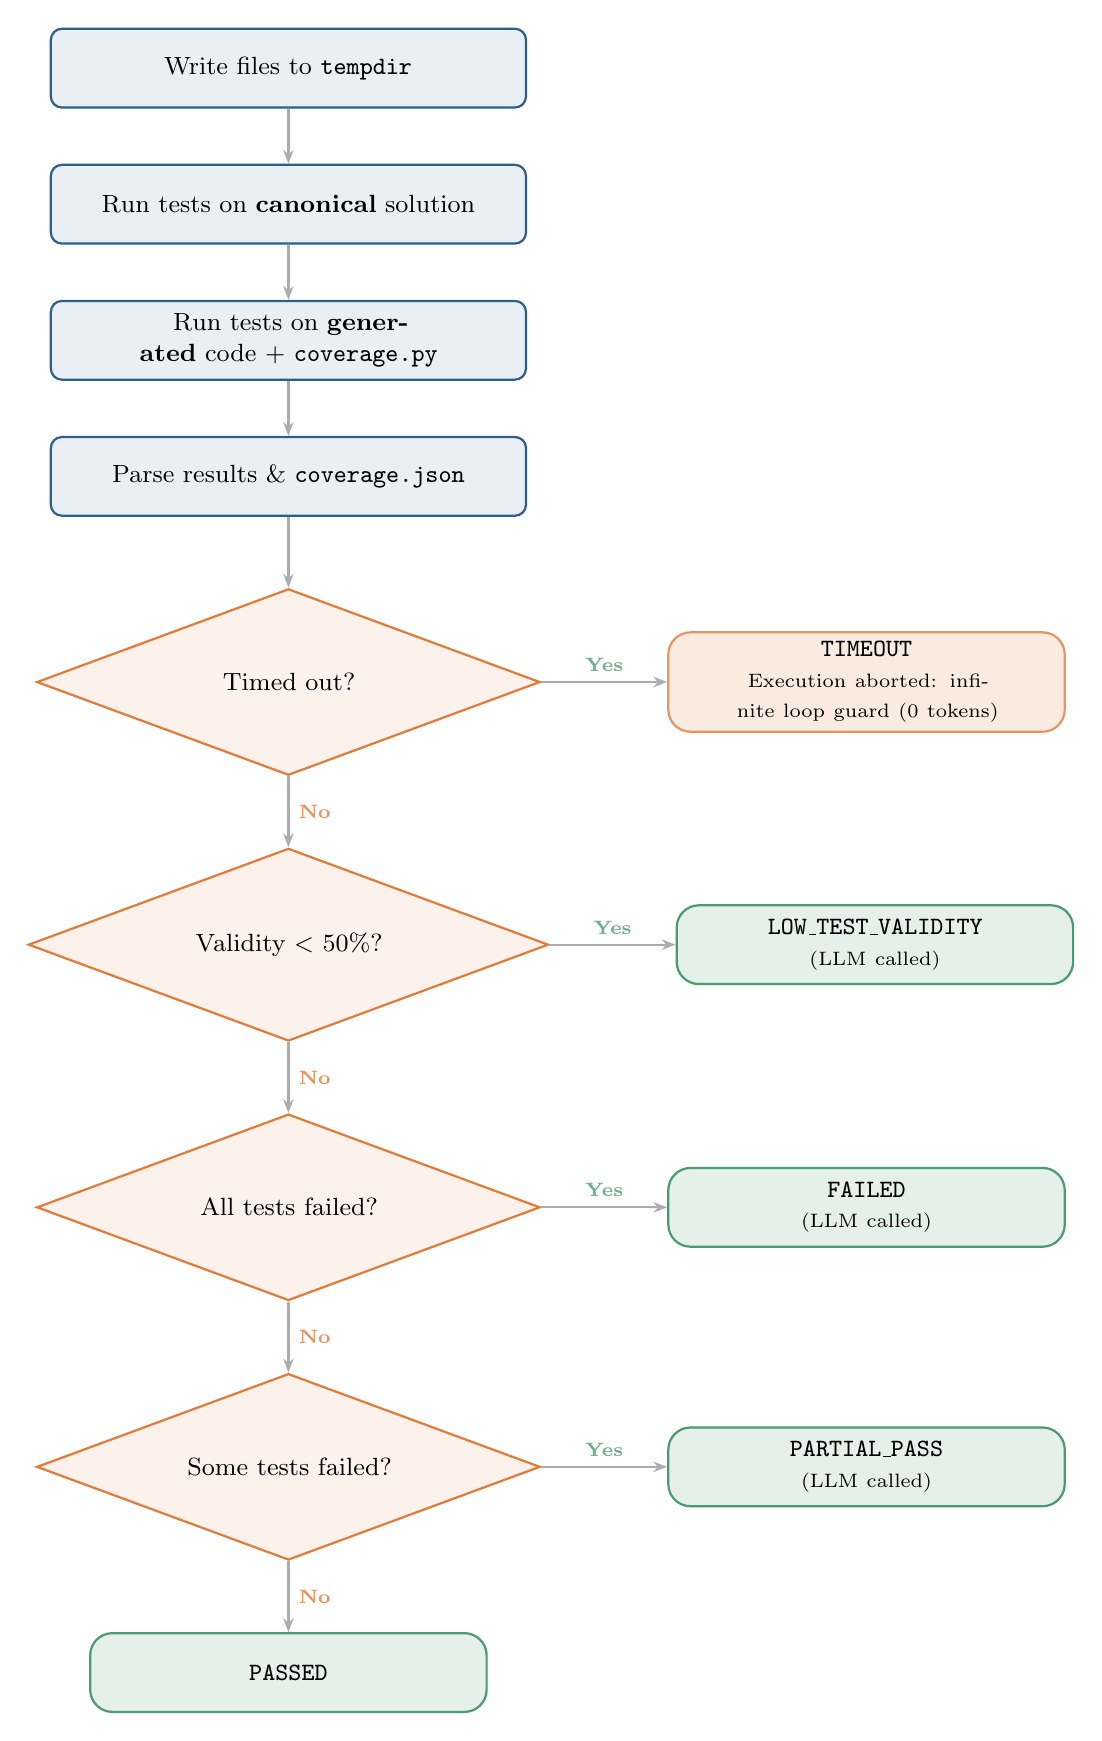
\begin{tikzpicture}[
  font=\small,
  node distance=7mm and 22mm,
  proc/.style={
    rectangle, rounded corners=4pt,
    minimum width=60mm, minimum height=10mm,
    text centered, text width=58mm,
    draw=AccentA, fill=AccentA!10, thick
  },
  dec/.style={
    diamond, aspect=2.7,
    minimum width=62mm, minimum height=10mm,
    text centered, text width=58mm,
    draw=AccentB, fill=AccentB!10, thick, inner sep=0pt
  },
  term/.style={
    rectangle, rounded corners=8pt,
    minimum width=50mm, minimum height=10mm,
    text centered, text width=48mm,
    draw=AccentC, fill=AccentC!15, thick
  },
  termhalt/.style={
    rectangle, rounded corners=8pt,
    minimum width=50mm, minimum height=10mm,
    text centered, text width=48mm,
    draw=AccentB!80, fill=AccentB!15, thick
  },
  arr/.style={-{Stealth[length=5pt]}, thick, color=gray!65},
  yes/.style={font=\scriptsize\bfseries, color=AccentC!80},
  no/.style={font=\scriptsize\bfseries, color=AccentB!80},
]

\node[proc] (p1) {Write files to \texttt{tempdir}};
\node[proc, below=of p1] (p2) {Run tests on \textbf{canonical} solution};
\node[proc, below=of p2] (p3) {Run tests on \textbf{generated} code + \texttt{coverage.py}};
\node[proc, below=of p3] (p4) {Parse results \& \texttt{coverage.json}};

\node[dec,  below=9mm of p4]   (d1) {Timed out?};
\node[termhalt, right=16mm of d1] (t1) {\textbf{\texttt{TIMEOUT}}\\\scriptsize Execution aborted: infinite loop guard (0 tokens)};

\node[dec,  below=9mm of d1]   (d2) {Validity $<$ 50\%?};
\node[term, right=16mm of d2]  (t2) {\textbf{\texttt{LOW\_TEST\_VALIDITY}}\\\scriptsize (LLM called)};

\node[dec,  below=9mm of d2]   (d3) {All tests failed?};
\node[term, right=16mm of d3]  (t3) {\textbf{\texttt{FAILED}}\\\scriptsize (LLM called)};

\node[dec,  below=9mm of d3]   (d4) {Some tests failed?};
\node[term, right=16mm of d4]  (t4) {\textbf{\texttt{PARTIAL\_PASS}}\\\scriptsize (LLM called)};

\node[term, below=9mm of d4]   (t5) {\textbf{\texttt{PASSED}}};

\draw[arr] (p1) -- (p2);
\draw[arr] (p2) -- (p3);
\draw[arr] (p3) -- (p4);
\draw[arr] (p4) -- (d1);
\draw[arr] (d1) -- node[yes, above]{Yes} (t1);
\draw[arr] (d1) -- node[no,  right]{No}  (d2);
\draw[arr] (d2) -- node[yes, above]{Yes} (t2);
\draw[arr] (d2) -- node[no,  right]{No}  (d3);
\draw[arr] (d3) -- node[yes, above]{Yes} (t3);
\draw[arr] (d3) -- node[no,  right]{No}  (d4);
\draw[arr] (d4) -- node[yes, above]{Yes} (t4);
\draw[arr] (d4) -- node[no,  right]{No}  (t5);

\end{tikzpicture}
\caption{Test Executor (Agent 3) -- internal verdict decision flowchart.}
\label{fig:executor}
\end{figure}

\subsubsection{Results for Demo Run (Task \#2)}

\begin{figure}[H]
\centering
\includegraphics[width=0.95\textwidth]{Buggy/metricsB.png}
\caption{Agent 3 output -- execution metrics and final verdict (Task \#2).}
\label{fig:metrics}
\end{figure}

\subsubsection{LLM Diagnostic Verdict}

\begin{figure}[H]
\centering
\includegraphics[width=0.95\textwidth]{Buggy/LLMVErdictB.png}
\caption{Agent 3 Phase 2 output -- LLM diagnostic failure triage verdict (Task \#2).}
\label{fig:llm-verdict}
\end{figure}

% ============================================================
\section{LLM Configuration and Parameters}
\label{sec:llm}
% ============================================================

\begin{table}[H]
\centering
\caption{LLM Model and API Configuration}
\begin{tabularx}{0.88\linewidth}{lX}
\toprule
\rowcolor{AccentA!10}
\textbf{Parameter} & \textbf{Value} \\
\midrule
Model name               & \texttt{nvidia/llama-3.1-nemotron-70b-instruct} \\
API endpoint             & \texttt{https://integrate.api.nvidia.com/v1}    \\
API compatibility        & OpenAI-compatible (via \texttt{openai} Python SDK) \\
Code gen.\ temperature   & 0.2 \\
Test gen.\ temperature   & 0.4 \\
LLM verdict temperature  & 0.2 \\
Execution timeout        & 5 seconds \\
\bottomrule
\end{tabularx}
\label{tab:llm}
\end{table}

The \texttt{LLMClient} class (\texttt{llm\_client.py}) is a thin wrapper around
the \texttt{openai} SDK configured for NVIDIA's hosted endpoint. Any
OpenAI-compatible endpoint (e.g.\ OpenRouter) can be substituted by updating
\texttt{NVIDIA\_BASE\_URL} in the \texttt{.env} file.

% ============================================================
\section{Code and Test Case Format}
\label{sec:format}
% ============================================================

\subsection{Generated Code}

Agent~1 produces a single, self-contained Python function. The LLM is instructed
to return only a \verb|```python ... ```| Markdown block; the
\texttt{LLMClient.extract\_code()} helper strips the fences via regex, leaving
clean, directly executable Python written to \texttt{solution.py} in the sandbox.

\begin{todobox}
Replace the placeholder listing below with the \textbf{actual generated Python
function} from your terminal run. Copy from the console block under
\texttt{--- Generated Code ---}.
\end{todobox}

\begin{lstlisting}[style=codestyle,
  caption={Generated code -- Task \#2 (replace with your actual output)}]
# TODO: Paste the actual generated function here.
def similar_elements(test_tup1, test_tup2):
    """Find similar elements from two tuples."""
    result = tuple(set(test_tup1) & set(test_tup2))
    return result
\end{lstlisting}

\subsection{Generated Test Suite}

Agent~2 produces a \texttt{unittest.TestCase} subclass. The executor prepends
\texttt{from solution import *} automatically if the test file does not already
contain an explicit import.

\begin{todobox}
Replace the placeholder listing below with the \textbf{actual generated test
class} from your terminal run. Copy from the console block under
\texttt{--- Generated Tests ---}.
\end{todobox}

\begin{lstlisting}[style=codestyle,
  caption={Generated test suite -- Task \#2 (replace with your actual output)}]
# TODO: Paste the actual generated test class here.
import unittest

class TestSolution(unittest.TestCase):

    def test_common_elements(self):
        self.assertEqual(
            set(similar_elements((3, 4, 5, 6), (5, 7, 4, 10))),
            {4, 5}
        )

    def test_no_common_elements(self):
        self.assertEqual(similar_elements((1, 2), (3, 4)), ())

    def test_identical_tuples(self):
        result = similar_elements((1, 2, 3), (1, 2, 3))
        self.assertEqual(set(result), {1, 2, 3})

    def test_empty_tuples(self):
        self.assertEqual(similar_elements((), ()), ())

if __name__ == '__main__':
    unittest.main(verbosity=2)
\end{lstlisting}

\subsection{Verdict Rules}

\begin{table}[H]
\centering
\caption{Verdict Decision Rules}
\begin{tabularx}{0.88\linewidth}{lX}
\toprule
\rowcolor{AccentA!10}
\textbf{Verdict} & \textbf{Condition} \\
\midrule
\texttt{TIMEOUT}             & Subprocess exceeded the 5-second limit \\
\texttt{LOW\_TEST\_VALIDITY} & Validity on canonical solution $<50\%$  \\
\texttt{PASSED}              & All tests pass on generated code \\
\texttt{PARTIAL\_PASS}       & Some (not all) tests pass \\
\texttt{FAILED}              & Zero tests pass on generated code \\
\bottomrule
\end{tabularx}
\label{tab:verdict}
\end{table}

% ============================================================
\section{Execution Results and Metrics}
\label{sec:results}
% ============================================================

\subsection{Coverage Criterion}

The pipeline pursues \textbf{coverage-based testing} (Requirement~1 from the
project specification). The test generator is explicitly prompted to achieve 100\%
statement and branch coverage on the generated code.

\subsection{Metrics}

\begin{table}[H]
\centering
\caption{Metrics Computed by the Pipeline}
\begin{tabularx}{0.92\linewidth}{llX}
\toprule
\rowcolor{AccentA!10}
\textbf{Metric} & \textbf{Tool} & \textbf{Description} \\
\midrule
Test Validity \%         & subprocess & \% of generated tests that pass against the
                                        \emph{canonical} solution \\
Statement Coverage \%    & coverage.py & \% of statements in the \emph{generated}
                                         function exercised by the tests \\
Generated Pass Rate \%   & subprocess & \% of tests that pass against the
                                        \emph{generated} function \\
Final Verdict            & Rule logic & Categorical outcome
                                        (\texttt{PASSED}, etc.) \\
\bottomrule
\end{tabularx}
\label{tab:metrics}
\end{table}

% ============================================================
\section{Project Structure}
\label{sec:structure}
% ============================================================

\begin{outputbox}{Directory Layout}
Project/
|-- .env                   (API key and model config)
|-- requirements.txt       (openai, coverage, python-dotenv)
|-- llm_client.py          (Shared LLM wrapper)
|-- main.py                (CLI entry point)
|-- agents/
|   |-- code_generator.py  (Agent 1)
|   |-- test_generator.py  (Agent 2)
|   `-- test_executor.py   (Agent 3: sandbox + coverage)
`-- data/
    |-- download_mbpp.py   (Dataset downloader)
    `-- sanitized-mbpp.json
\end{outputbox}

\textbf{Dependencies (requirements.txt):}
\begin{itemize}[leftmargin=18pt, itemsep=2pt]
  \item \texttt{openai $\geq$ 1.0.0} --- LLM API communication
  \item \texttt{coverage $\geq$ 7.0.0} --- Statement and branch coverage
  \item \texttt{python-dotenv $\geq$ 1.0.0} --- Environment variable management
\end{itemize}

% ============================================================
\section{Design Decisions}
\label{sec:design}
% ============================================================

\begin{itemize}[leftmargin=18pt, itemsep=5pt]

  \item \textbf{No orchestration frameworks.} The pipeline uses only standard
        Python, honouring the course requirement to build from first principles.

  \item \textbf{Subprocess sandbox.} Agent~3 uses \texttt{tempfile} +
        \texttt{subprocess} instead of \texttt{exec()} or \texttt{eval()}, so
        untrusted generated code cannot affect the host process.

  \item \textbf{Dual evaluation.} Tests run against both the canonical solution
        (validity check) and the generated code (coverage + pass rate), providing
        a two-dimensional quality signal.

  \item \textbf{Coverage via \texttt{coverage.py}.} Invoked as a subprocess with
        \texttt{--branch} mode; its JSON report is parsed to extract percentages
        reliably.

  \item \textbf{Differentiated temperatures.} Code generation uses $T=0.2$
        (deterministic, correct output); test generation uses $T=0.4$ (varied,
        creative output) to maximise test diversity and coverage.

\end{itemize}

% ============================================================
\section{Conclusion}
\label{sec:conclusion}
% ============================================================

This project shows that a compact three-agent pipeline --- built without any
third-party orchestration framework --- can meaningfully automate unit test
generation and evaluation. Separating code generation, test generation, and test
execution into distinct agents, each with tailored prompts and temperature
settings, produces tests that achieve high statement coverage and strong test
validity scores on MBPP problems.

The dual-execution strategy and subprocess sandbox ensure both safety and a
clear two-dimensional quality signal for every pipeline run.

% ============================================================
\section{Team Contributions}
\label{sec:contributions}
% ============================================================

\begin{table}[H]
\centering
\caption{Individual Contributions}
\begin{tabularx}{0.92\linewidth}{lX}
\toprule
\rowcolor{AccentA!10}
\textbf{Member} & \textbf{Contributions} \\
\midrule
% TODO: Replace with actual names and real contributions
Name of Member 1 &
  Dataset integration (\texttt{download\_mbpp.py}),
  \texttt{LLMClient} design,
  \texttt{CodeGeneratorAgent}, \texttt{TestGeneratorAgent},
  prompt engineering, \texttt{main.py} \\
\addlinespace
Name of Member 2 &
  \texttt{TestExecutorAgent} (subprocess sandbox,
  \texttt{coverage.py} integration, verdict logic, LLM verdict),
  testing and debugging, report writing \\
\bottomrule
\end{tabularx}
\label{tab:contributions}
\end{table}

\end{document}
